\documentclass[../opis-rozwiazania.tex]{subfiles}

\begin{document}
\label{system_interaction}

\subsection{Typowe działanie systemu}
Po uruchomieniu opisanym w \ref{system_startup.procedure} system powinien być w pełni używalny.
Typowym zachowaniem systemu będzie cykliczne wysyłanie próśb przez nadzorców do serwerów wirtualizacji.
W logach serwerów wirtualizacji jak i nadzorców powinny cyklicznie pojawiać się informacje o prośbie lub odpowiedzi na zapytanie o model.

Zaraz po starcie systemu powinny pojawić się prośby u włączenie maszyn wirtualnych na odpowiednich serwerach wirtualizacji.
Przy patrzeniu na standardowe wyjście aplikacji powinny być widoczne informacje od uruchamiającego się Vagranta.
Przy każdej nowej utworzonej sesji powinny wybudzać się następne maszyny wirtualne.
Często problemy z uruchomieniem maszyn wirtualnych będą oznaczać nieskończone próby uruchamiania maszyn wirtualnych, które zawsze będą kończyć się niepowodzeniem.
Serwer wirtualizacji powinien wszystkie informacje o błędach zapisywać do pliku z logami we wnętrzu kontenera w folderze roboczym aplikacji \texttt{/app}.

Przy wyłączaniu serwerem wirtualizacji mogą pozostać nadal działające maszyny wirtualne wytworzone przez niego.
Maszyny takie należy ręcznie wyłączyć lub usunąć.
Nazwy maszyn można wyczytać z logów pracy serwera wirtualizacji.

\subsection{Funkcje panelu administracyjnego}

Po wejściu na stronę panelu administracyjnego administrator musi podać nazwę użytkownika i hasło.
Jeżeli rzeczywiście podane konto jest kontem administratora przejdzie dalej do panelu.
W przeciwnym wypadku zostanie zwrócony błąd dostępu.

\begin{figure}[H]
	\centering
	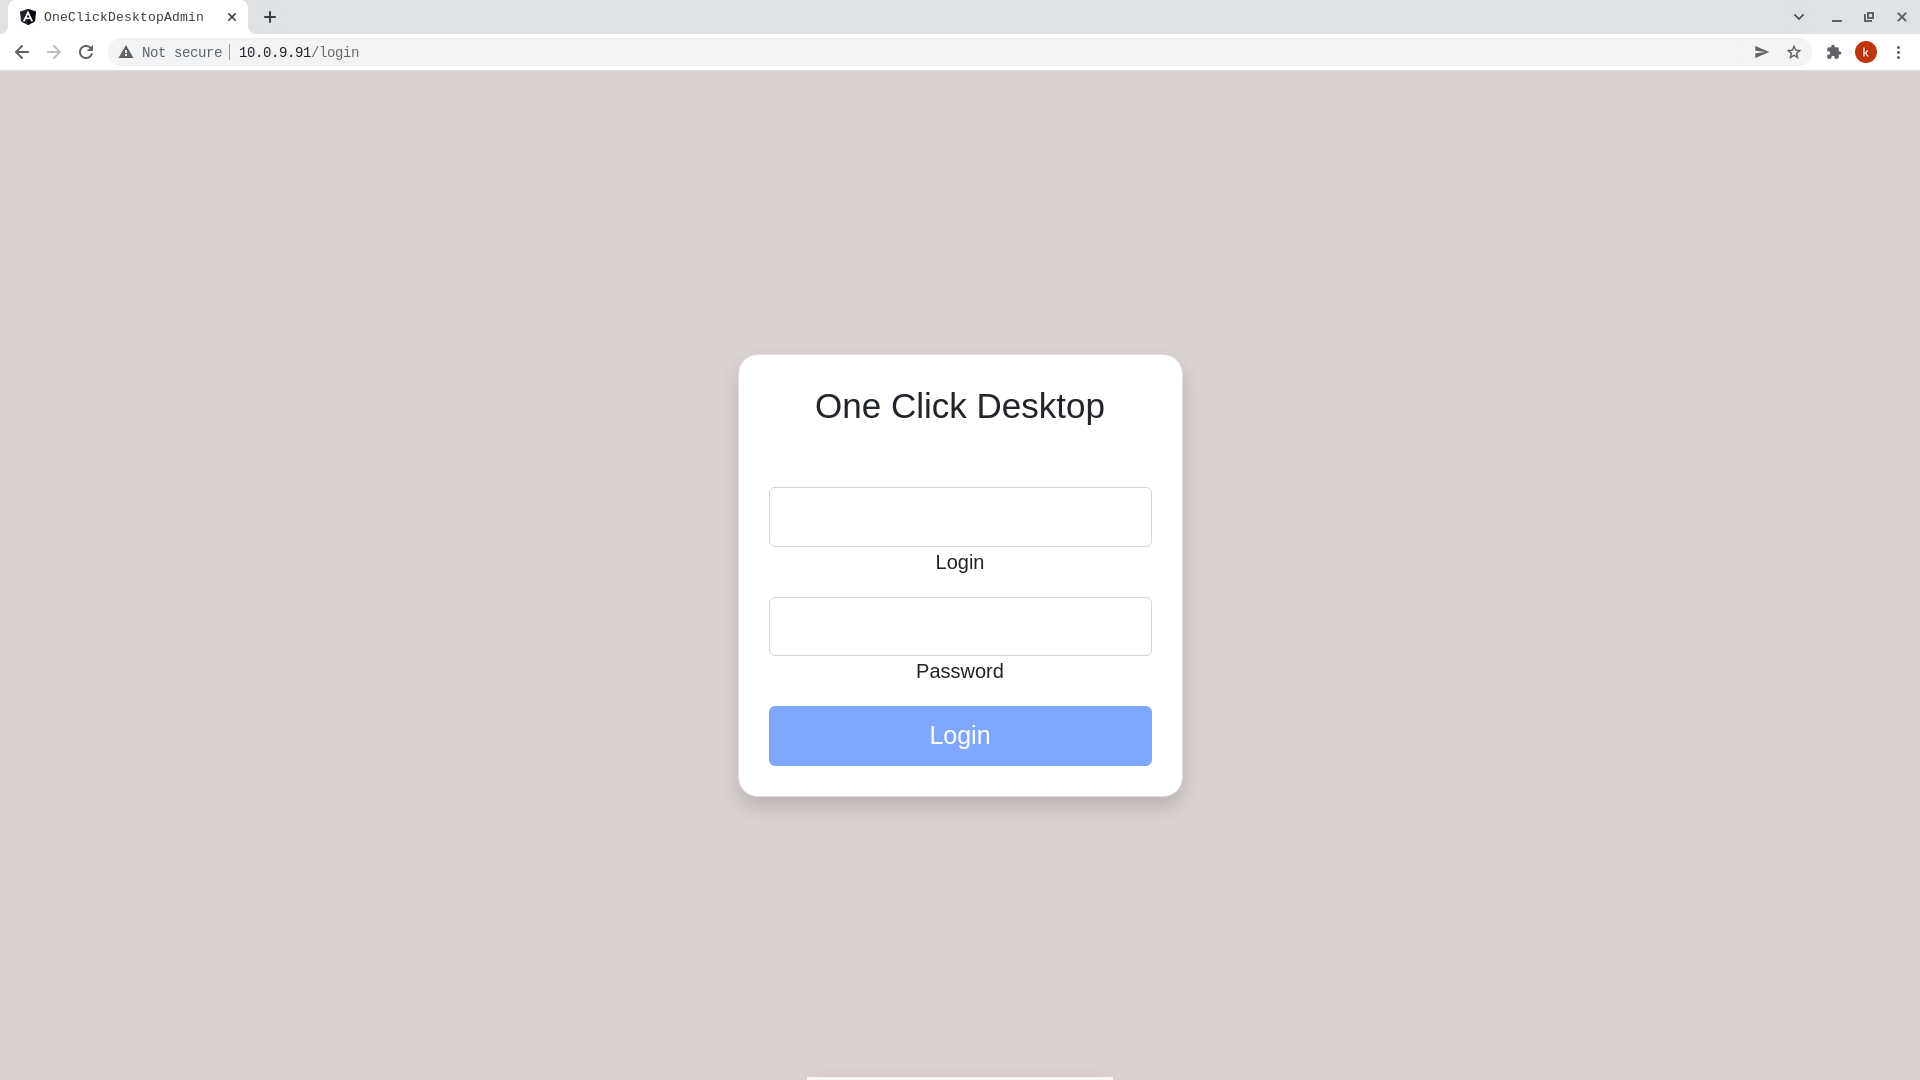
\includegraphics[width=\textwidth]{resources/admin_panel_login.png}
	\caption{Okno logowania panelu administracyjnego}
	\label{figure:system_interaction.admin.login}
\end{figure}

Po zalogowaniu administrator ma dostęp do głównego panelu z podsumowaniem wszystkich dostępnych zasobów.
Po lewej stronie ma on dostępna listę wszystkich aktywnych serwerów wirtualizacji w systemie (rysunek \ref{figure:system_interaction.admin.panel}).

\begin{figure}[H]
	\centering
	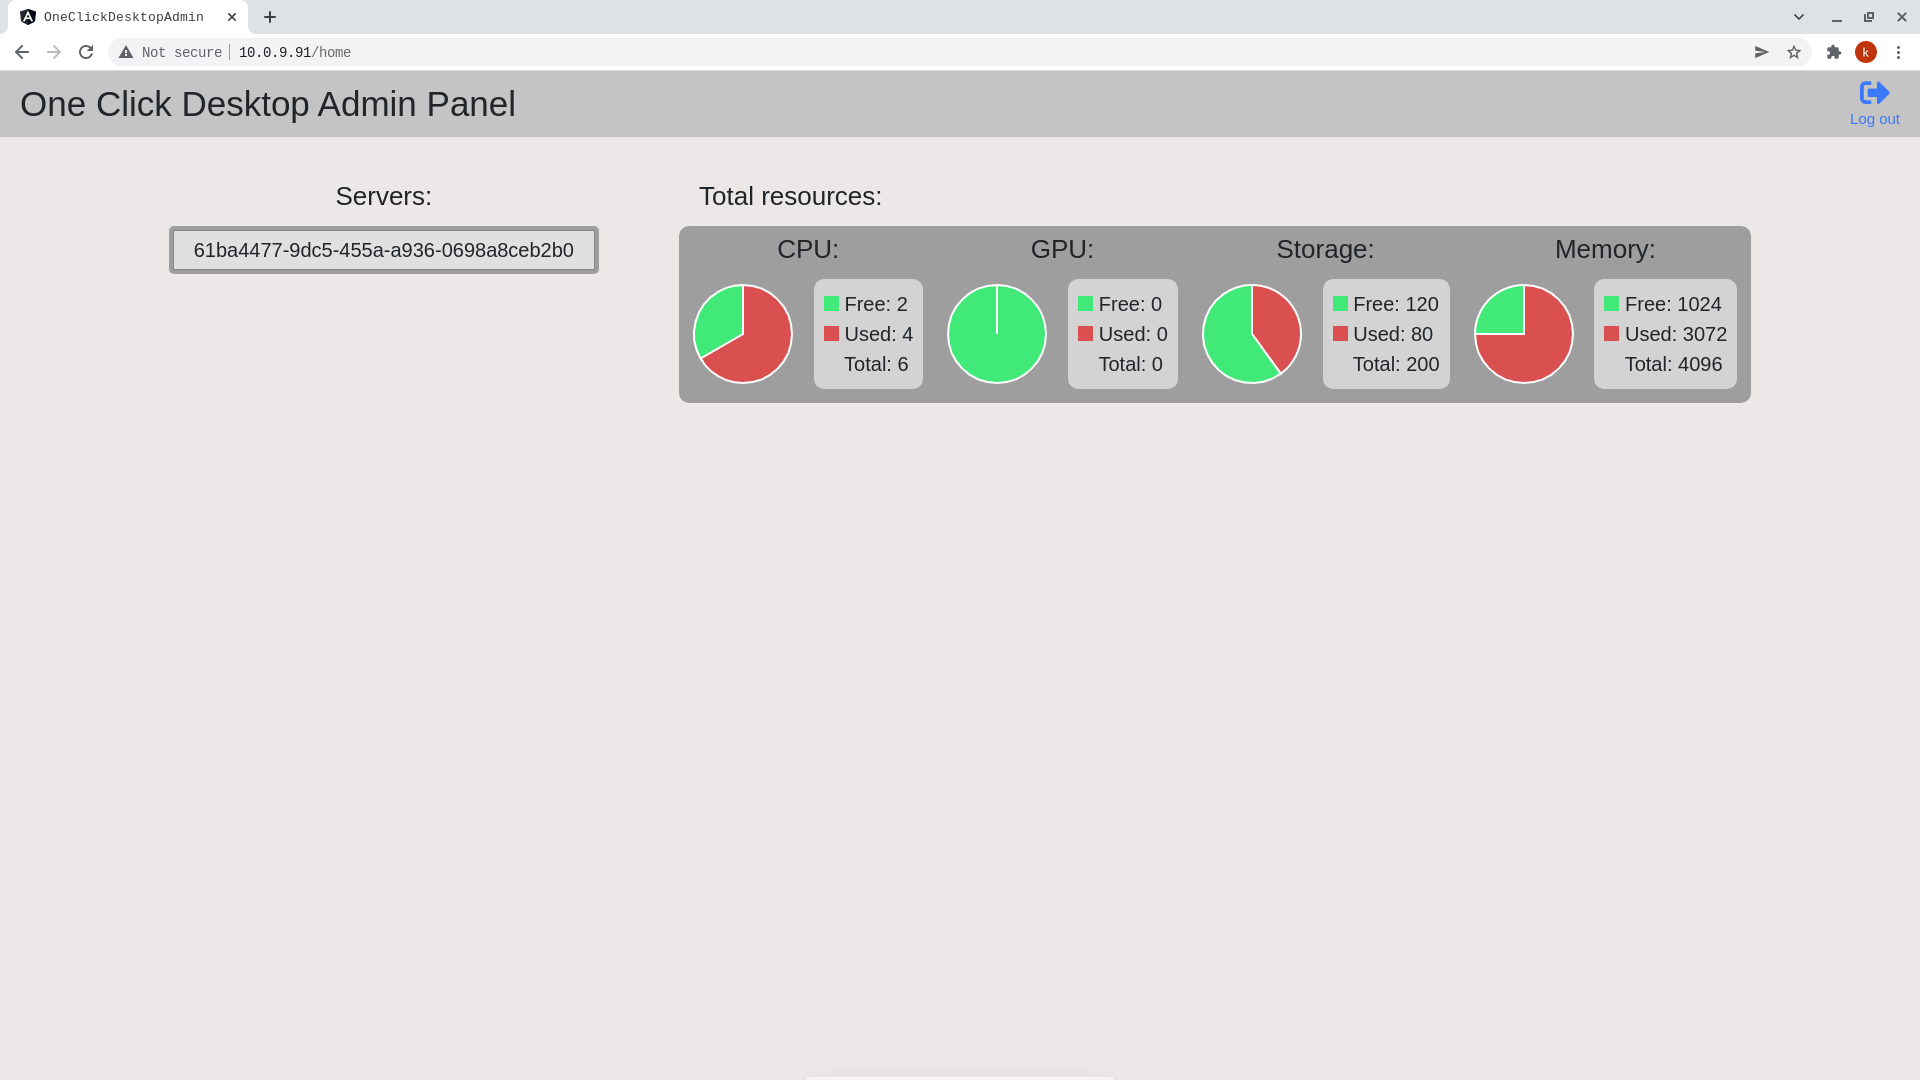
\includegraphics[width=\textwidth]{resources/admin_panel_home.png}
	\caption{Widok wszystkich zasobów systemu}
	\label{figure:system_interaction.admin.panel}
\end{figure}

Po naciśnięciu na wybrany serwer wirtualizacji na środku pojawiają się szczegóły zasobów konkretnego serwera (rysunek \ref{figure:system_interaction.admin.details}).
Administrator Oprócz zasobów może sprawdzić ile aktualnie jest uruchomionych maszyn (sekcja Running) oraz ile maszyn można jeszcze uruchomić (sekcja Free).

\begin{figure}[H]
	\centering
	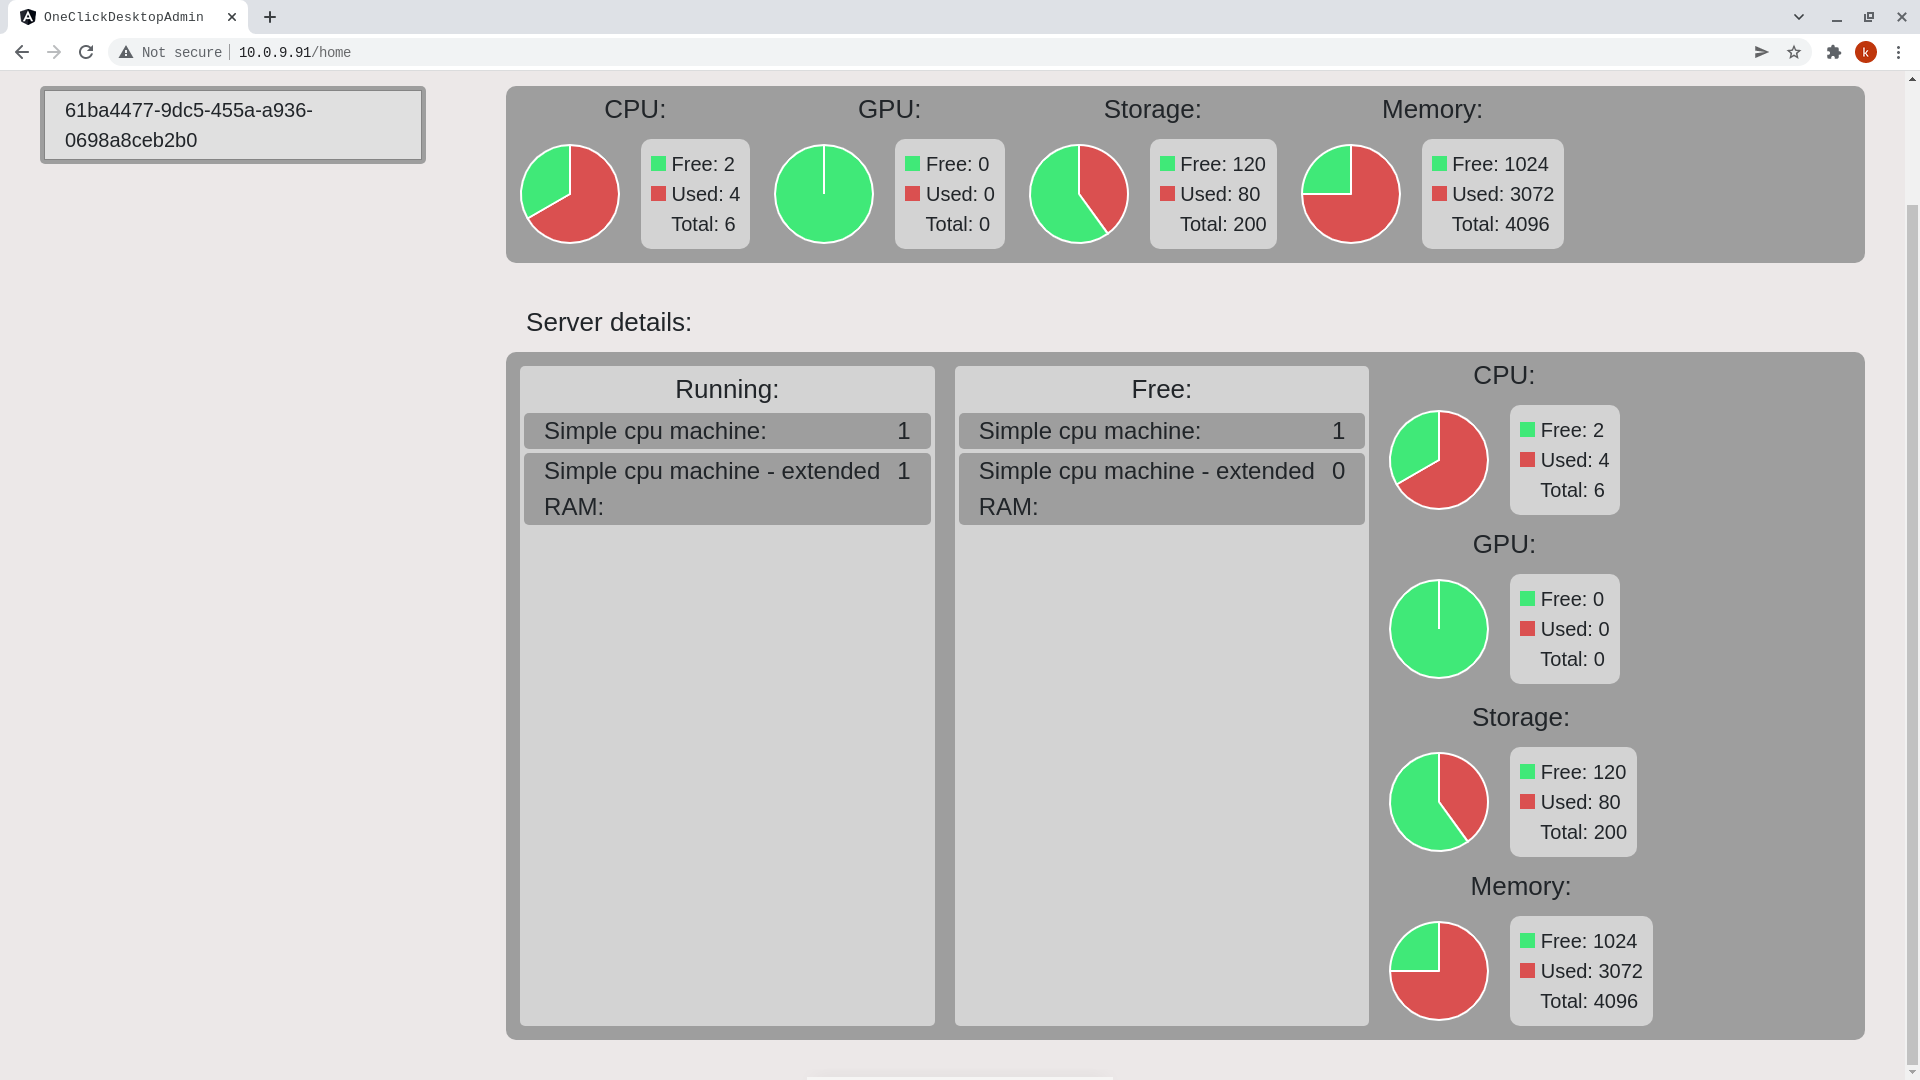
\includegraphics[width=\textwidth]{resources/admin_panel_details.png}
	\caption{Widok szczegółowych zasobów serwera wirtualizacji}
	\label{figure:system_interaction.admin.details}
\end{figure}

Zawartość panelu odświeża się automatycznie.

\newpage
\subsection{Funkcje aplikacji klienckiej}

Po uruchomieniu aplikacji klienckiej użytkownik musi podać nazwę użytkownika i hasło.
Jeżeli użytkownik istnieje w bazie to przejdzie do ekranu podsumowania.
W przeciwnym wypadku zostanie zwrócony błąd dostępu.

\begin{figure}[H]
	\centering
	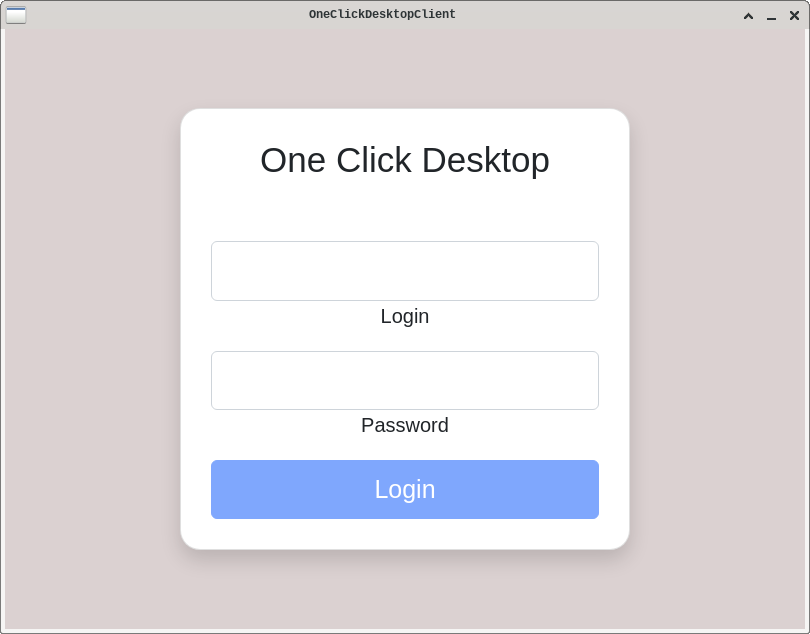
\includegraphics[width=\textwidth]{resources/client_login.png}
	\caption{Ekran logowania aplikacji klienckiej}
	\label{figure:system_interaction.client.login}
\end{figure}

Po zalogowaniu użytkownik trafia do ekranu głównego (rysunek \ref{figure:system_interaction.client.home}).
Może tutaj zobaczyć ile jest dostępnych maszyn w systemie, poprosić o sesję oraz zmienić ustawienia aplikacji.

\begin{figure}[H]
	\centering
	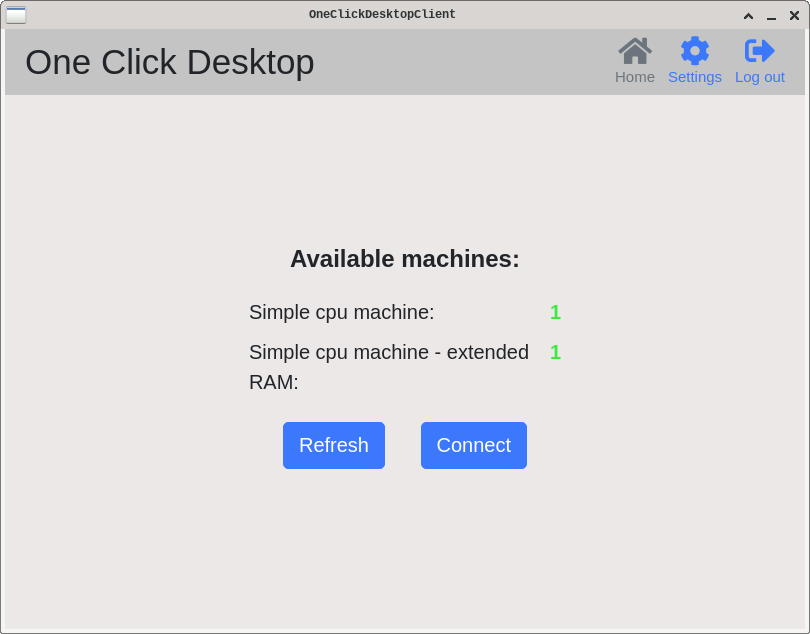
\includegraphics[width=\textwidth]{resources/client_home.png}
	\caption{Ekran główny aplikacji klienckiej}
	\label{figure:system_interaction.client.home}
\end{figure}

Przechodząc do ustawień (rysunek \ref{figure:system_interaction.client.settings}) użytkownik może edytować plik konfiguracyjny z poziomu aplikacji albo wrócić do ekranu głównego.
Zmiana adresu do nadzorcy będzie wymagać ponownego uruchomienia.
Inne ustawienia zostaną zastosowane od razu po zmianie.

\begin{figure}[H]
	\centering
	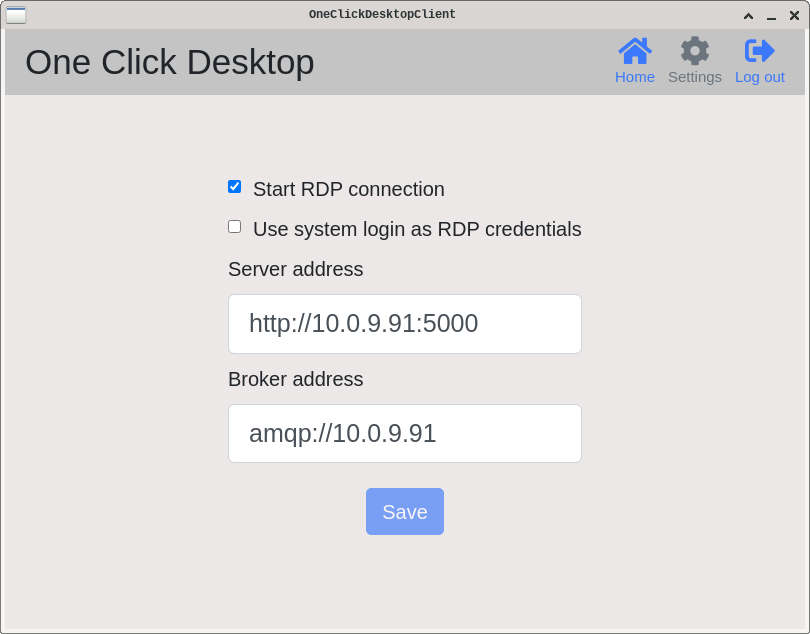
\includegraphics[width=\textwidth]{resources/client_settings.png}
	\caption{Ekran ustawień aplikacji klienckiej}
	\label{figure:system_interaction.client.settings}
\end{figure}

Gdy użytkownik z ekranu głównego naciśnie przycisk \textit{Connect} zostanie zapytany o typ sesji, jaki system am mu przypisać (rysunek \ref{figure:system_interaction.client.select}).

\begin{figure}[H]
	\centering
	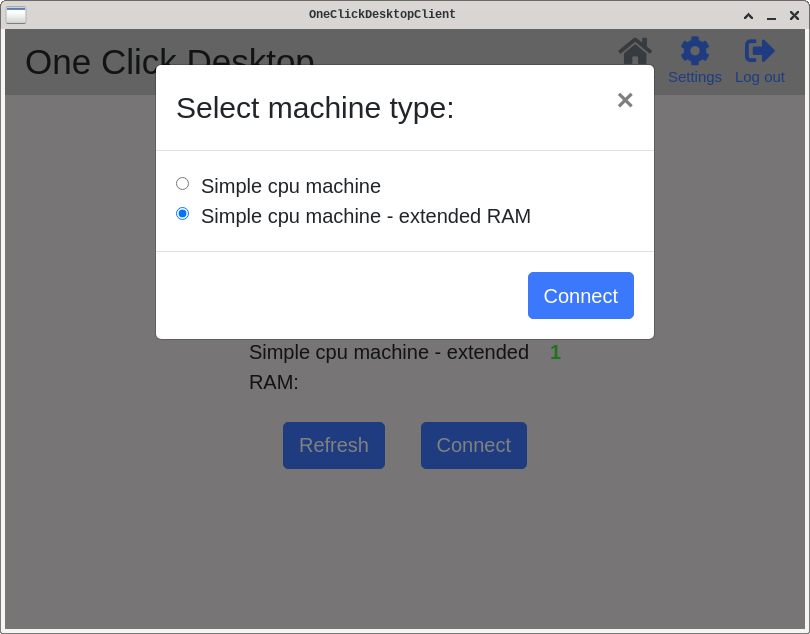
\includegraphics[width=\textwidth]{resources/client_select.png}
	\caption{Ekran wyboru typu maszyny do pracy}
	\label{figure:system_interaction.client.select}
\end{figure}

Po wybraniu jednego z typów sesji i naciśnięciu przycisku \textit{Connect} aplikacja kliencka wyślę prośbę o znalezienie maszyny danego typu i utworzenie sesji dla pytającego użytkownika.
Do czasu utworzenia sesji aplikacja będzie oczekiwać na dane do połączenia.
W przypadku poprawnego utworzenia sesji uruchomi się klient RDP i będzie można rozpocząć pracę.
W przeciwnym wypadku zostanie zgłoszony błąd i prośba o sesję zostanie umorzona.

Po prawidłowym utworzeniu sesji aplikacja rozpocznie zgłaszanie do zewnętrznego brokera wiadomości, że użytkownik pracuje na maszynie wirtualnej.
Ten stan reprezentuje ekran pokazany na rysunku \ref{figure:system_interaction.client.session}.
Zamknięcie klienta RDP albo naciśniecie przycisku \textit{End session} spowoduje oznaczenie sesji jako \textit{do usunięcia}.
Od tego momentu użytkownik ma \texttt{DomainShutdownTimeout} minut na powrót do swojej sesji (szczegóły w \ref{system_startup.overseer_conf}).
Po upływie tego czasu sesja zostaje zamknięta oraz maszyna z nią skojarzona wyłączona.

\begin{figure}[H]
	\centering
	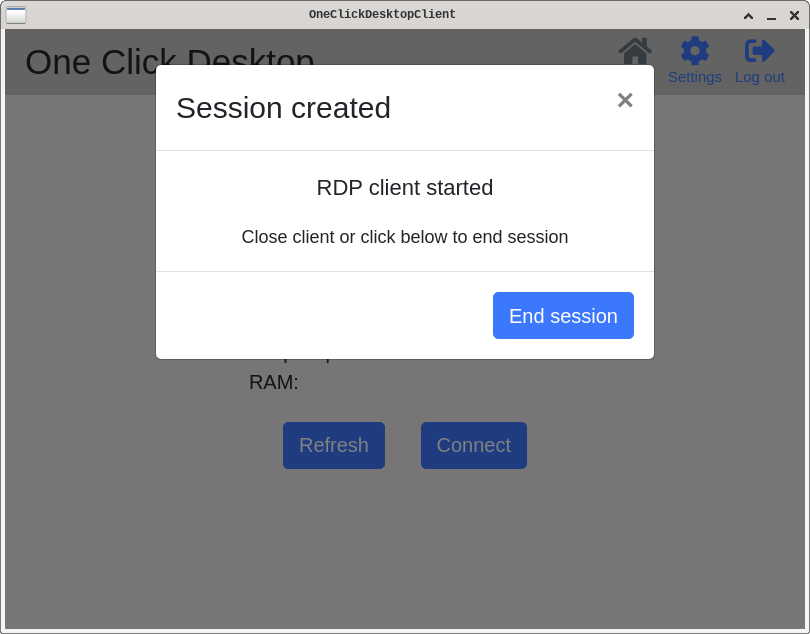
\includegraphics[width=\textwidth]{resources/client_session.png}
	\caption{Ekran działającego połączenia RDP}
	\label{figure:system_interaction.client.session}
\end{figure}

W przypadku, gdy użytkownik poprosi aby nie uruchamiać dołączonego klienta RDP albo uruchomieni klienta RDP zakończy się błędem zostaną mu przekazane dane dostępowe do przypisanej maszyny wirtualnej (rysunek \ref{figure:system_interaction.client.session_nordp}).
Wtedy jedynym sposobem na zaznaczenie, że skończyło się prace na maszynie, jest naciśniecie przycisku \textit{End session}.

\begin{figure}[H]
	\centering
	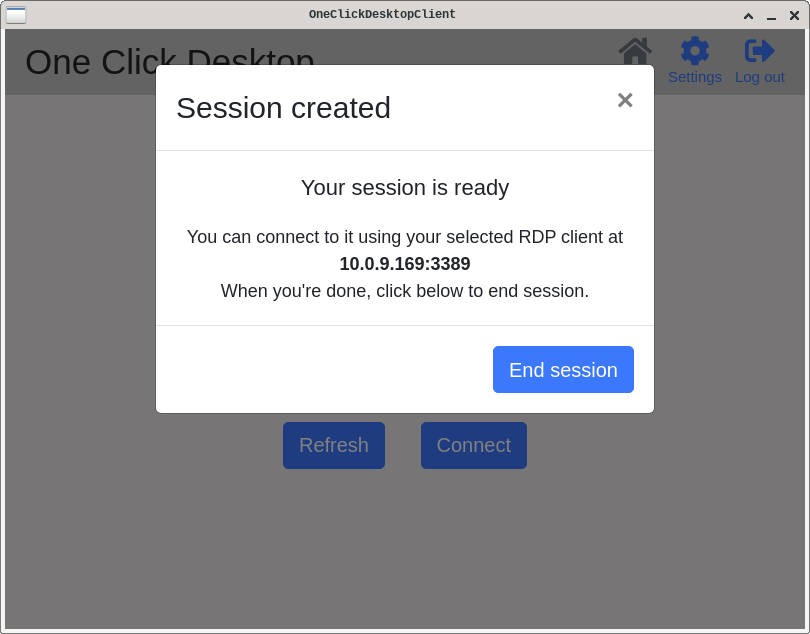
\includegraphics[width=\textwidth]{resources/client_session_nordp.png}
	\caption{Ekran trwania połączenia w zewnętrznym kliencie RDP}
	\label{figure:system_interaction.client.session_nordp}
\end{figure}


\end{document}